\section{Limitaciones conocidas de los LLM}
\label{sec:limitaciones_llm}

\cite{arunbijiRAGVsFinetuning} enumera una serie de limitaciones que actualmente muestran los \gls{llm} y que consideramos muy importantes a la hora de valorar su uso en el contexto de este trabajo. Estas limitaciones son:

\subsection{Corte de conocimiento}

Los \gls{llm} no aprenden nuevos datos tras su entrenamiento, por lo que existe una limitación en la información o el conocimiento disponible por no haber tenido acceso a información o acontecimientos ocurridos después de esa fecha límite. Esta limitación se minimiza con rentrenamientos tipo \emph{fine-tuning} o con técnicas como \gls{rag}.

\subsection{Alucinaciones}
\label{sec:alucinaciones}

Se entiende por \emph{alucinación} a un dato erróneo que el modelo genera con total apariencia de verosimilitud y corrección. Para entender por qué sucede esto, hay que comprender que la finalidad de un \gls{lm} es \emph{modelar} el lenguaje humano, por lo que, a priori, no se puede esperar que los datos que devuelva en sus respuestas sean ciertos, sino solo verosímiles. Los \gls{llm} se entrenan con vastas cantidades de datos de diversa calidad, y la trazabilidad de los datos que devuelve en sus respuestas es muy difícil de determinar. Precisamente, la técnica \gls{rag} permite dibujar dicha trazabilidad de los datos de las respuestas, en tanto en cuanto estas se basan en los datos de la base de datos de conocimiento. Por otra parte, la constante mejora de los datos de entramiento de los \gls{llm} \citep{gunasekarTextbooksAreAll2023} hace que este problema de las alucinaciones se minimice aunque nunca se elimina completamente.

\subsection{Ineficiencia y coste}

Una de las razones por las que los \gls{llm}, y toda la \gls{iag} en general, no se ha desarrollado hasta hace relativamente poco tiempo, es la alta demanda de recursos computacionales que requiere tanto su fase de entrenamiento como su fase de inferencia. La carrera actual en el desarrollo de la \gls{ia} reside en ganar eficiencia en los modelos. 

Los problemas de eficiencia y coste se pueden articular en torno a tres ejes \citep{arunbijiRAGVsFinetuning}:

\begin{enumerate}[label=\alph*)]
    \item \textit{Recursos de tiempo computacional:} El tiempo necesario para entrenar un \gls{llm} es muy alto, y depende del tamaño del modelo, del conjunto de datos de entrenamiento y de la capacidad de cómputo disponible. En general, se habla en términos de \emph{años de GPU}, lo cual está fuera del alcance de la computación de usuario. La Figura \ref{fig:llm_gpu_training_hours} muestra el coste en millones de horas de GPU de diversos modelos de lenguaje de código abierto. En la fase de inferencia el coste computacional, aunque menor que en la fase de entrenamiento, sigue siendo alto, lo cual constituye un problema para el uso de \gls{llm} en local en dispositivos de usuario final.
    \item \textit{Recursos de memoria:} No es el tiempo de procesador el único origen de la ineficiencia. Estos modelos, de tamaños gigantescos, requieren de grandes cantidades de memoria RAM para su entrenamiento e inferencia. En \gls{llm} \emph{open source} como Mistral o LLamA, en versiones comparables en rendimiento a GPT-3.5, se necesita entre 16 y 100 GB en GPU para la inferencia. 
    \item \textit{Recursos económicos:} Finalmente, los costes computacionales se traducen en costes económicos, solo asumibles por grandes corporaciones. De ahí que la mayoría de \gls{llm} sean propiedad de empresas como Google, Facebook o Microsoft, quienes los ponen a disposición de los usuarios a través de sus \gls{api}.
\end{enumerate}

\begin{figure}[H]
    \caption[Coste de entrenamiento en horas de GPU de diversos modelos de lenguaje]{Coste de entrenamiento en horas de GPU de diversos modelos de lenguaje.}
    \centering
    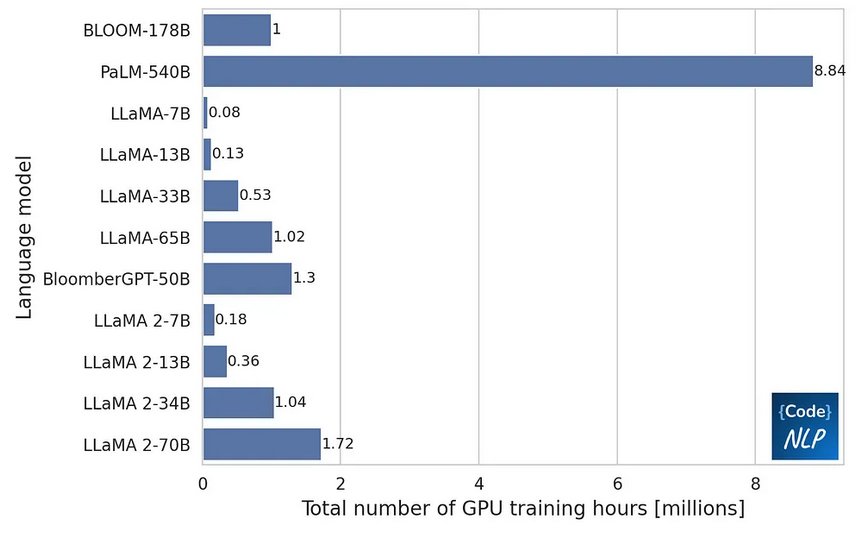
\includegraphics[width=0.6\textwidth]{./figuras/llm_gpu_training_hours.png}
    \source{\cite{ph.dTrainingTimeFoundation2023}}
    \label{fig:llm_gpu_training_hours}
  \end{figure}

Es de esperar que la eficiencia de recursos mejore con el tiempo. De hecho, ya se están viendo significativos avances en este sentido, especialmente de la mano del \emph{open source}, que está democratizando el acceso a los \gls{llm} y a la \gls{ia} en general, con sus contribuciones a mejoras en la arquitectura de los modelos, su proceso de entrenamiento, la eficiencia en dispositivos de bajos recursos y la creación de conjuntos de datos de entrenamiento de alta calidad, entre otros. En estos momentos, la gran mayoría de modelos de código abierto que grandes empresas crean y entrenan, y los propios usuarios rentrenan con un \emph{fine-tuning}, se pueden descargar y utilizar de forma gratuita desde repositorios como \href{https://huggingface.co/}{Hugging Face}.


\subsection{Modelos de \emph{caja negra}, con sesgos y riesgos}

Los \gls{llm} funcionan como modelos de \emph{caja negra}, lo que significa que los detalles internos de su proceso de generación de respuestas son inaccesibles incluso por sus creadores. Esta característica se debe a su naturaleza probabilística, donde la generación de texto se basa en la probabilidad de secuenciación de tokens y no en una serie de reglas predefinidas. Por consiguiente, es imposible discernir el procedimiento específico que emplea el modelo para elaborar sus respuestas. Esta limitación ha de ser tenida en consideración en el contexto de los \gls{llm}, que se distinguen de otros modelos de \gls{ia}, como los de clasificación, en que no se entrenan mediante datos etiquetados, sino que desarrollan su aprendizaje de manera autónoma a partir de grandes volúmenes de datos no etiquetados.

La falta de transparencia en los \gls{llm} conlleva la especial dificultad de identificar cualquier sesgo inherente al modelo. La opacidad y el sesgo de los \gls{llm} no solo plantean dilemas éticos, sino que también constituyen un riesgo potencial de seguridad, consideración importante en el contexto de nuestro estudio.